%%%%%%%%%%%%%%%%%%%%%%%%%%%%%%%%%%%%%%%%%%%%%%%%%%%%%%%%%%%%%%%%%%%%%%%
%%%%%%%%%%%%%%%%%%%%%%%%%%%%%%%%%%%%%%%%%%%%%%%%%%%%%%%%%%%%%%%%%%%%%%% 
%%%%%%%%%%%       								 Preamble				         	                                                        %%%%%%%%%% 
%%%%%%%%%%%%%%%%%%%%%%%%%%%%%%%%%%%%%%%%%%%%%%%%%%%%%%%%%%%%%%%%%%%%%%% 
%%%%%%%%%%%%%%%%%%%%%%%%%%%%%%%%%%%%%%%%%%%%%%%%%%%%%%%%%%%%%%%%%%%%%%% 
\documentclass[10pt]{beamer}
\usepackage{setspace}
\usepackage{color}
\usepackage{amsmath,lmodern}
\usepackage{hyperref}
\usepackage{graphicx}
\usepackage{multirow}
\usepackage{tikz}
\usetikzlibrary{fit,shapes.misc}
\usepackage{pdflscape}
\usepackage{amsmath}
\usepackage{lscape}
\usepackage{multirow}
\usepackage{enumerate}
\usepackage{epstopdf}
\usepackage{pdfpages}
\usepackage{appendixnumberbeamer}
\usepackage{color,soul}
\usepackage{grffile}
\usepackage{float}
\usepackage{relsize}
\usepackage{tcolorbox}
\newcounter{nodemarkers}
\usepackage{tikz}
\newcommand{\toplinesmall}{%
  \tikz[remember picture,overlay] {%
    \draw[blue,thick] ([yshift=-1cm, xshift=.9cm]current page.north west)
             -- ([yshift=-1cm,xshift=3.6cm]current page.north west);}}
             
\newcommand{\toplinemedium}{%
  \tikz[remember picture,overlay] {%
    \draw[blue,thick] ([yshift=-1cm, xshift=.9cm]current page.north west)
             -- ([yshift=-1cm,xshift=6.2cm]current page.north west);}}
 
 \newcommand{\toplinelarge}{%
  \tikz[remember picture,overlay] {%
    \draw[blue,thick] ([yshift=-1cm, xshift=.9cm]current page.north west)
             -- ([yshift=-1cm,xshift=8.9cm]current page.north west);}}           
             
 \newcommand{\toplinexlarge}{%
  \tikz[remember picture,overlay] {%
    \draw[blue,thick] ([yshift=-1cm, xshift=.9cm]current page.north west)
             -- ([yshift=-1cm,xshift=12cm]current page.north west);}}                       
             
\setbeamertemplate{footline}
{
  \leavevmode%
  \hbox{%
  \begin{beamercolorbox}[wd=.333333\paperwidth,ht=2.25ex,dp=1ex,center]{author in head/foot}%
    \usebeamerfont{author in head/foot}{\textcolor{blue}{ECON311}}
  \end{beamercolorbox}%
  \begin{beamercolorbox}[wd=.333333\paperwidth,ht=2.25ex,dp=1ex,center]{title in head/foot}%
    \usebeamerfont{title in head/foot}{\textcolor{blue}{Winter 2026}}
  \end{beamercolorbox}%
  \begin{beamercolorbox}[wd=.333333\paperwidth,ht=2.25ex,dp=1ex,right]{date in head/foot}%
    \usebeamerfont{date in head/foot}{\textcolor{blue}{Lecture 13\: \: \: \: \: \: \: }
    \insertframenumber{} / \inserttotalframenumber\hspace*{2ex}} 
  \end{beamercolorbox}}%
  \vskip0pt%
}
\newtheorem{proposition}[theorem]{Proposition}

\newcommand\marktopleft[1]{%
    \tikz[overlay,remember picture] 
        \node (marker-#1-a) at (-0.2,1.2ex) {};%
}
\newcommand\markbottomright[1]{%
    \tikz[overlay,remember picture] 
        \node (marker-#1-b) at (0.16,-1ex) {};%
    \tikz[overlay,remember picture,thick,inner sep=4pt]
        \node[draw,rectangle,rounded corners, blue, fit=(marker-#1-a.center) (marker-#1-b.center)] {};%
}

\setbeamertemplate{caption}{\raggedright\insertcaption\par}
\setbeamertemplate{itemize items}[ball]
\setbeamertemplate{itemize subitem}[triangle]
\setbeamertemplate{itemize subsubitem}[triangle]
\tcbset{colframe=white,colback=white,nobeforeafter}
\beamertemplatenavigationsymbolsempty
\addtobeamertemplate{frametitle}{\vspace*{0.19cm}}{\vspace*{0cm}}


%%%%%%%%%%%%%%%%%%%%%%%%%%%%%%%%%%%%%%%%%%%%%%%%%%%%%%%%%%%%%%%%%%%%%%%
%%%%%%%%%%%%%%%%%%%%%%%%%%%%%%%%%%%%%%%%%%%%%%%%%%%%%%%%%%%%%%%%%%%%%%% 
%%%%%%%%%  									    Define Title									                                       %%%%%%%%%
%%%%%%%%%%%%%%%%%%%%%%%%%%%%%%%%%%%%%%%%%%%%%%%%%%%%%%%%%%%%%%%%%%%%%%%
%%%%%%%%%%%%%%%%%%%%%%%%%%%%%%%%%%%%%%%%%%%%%%%%%%%%%%%%%%%%%%%%%%%%%%% 
\title{ECON 311} 
\author{Lecture 13: The IS-MP Model, part II}
\date{}
\AtBeginSection[]
{
 \begin{frame}<beamer>
 \tableofcontents[currentsection]
 \end{frame}
}
%%%%%%%%%%%%%%%%%%%%%%%%%%%%%%%%%%%%%%%%%%%%%%%%%%%%%%%%%%%%%%%%%%%%%%%
%%%%%%%%%%%%%%%%%%%%%%%%%%%%%%%%%%%%%%%%%%%%%%%%%%%%%%%%%%%%%%%%%%%%%%% 
%%%%%%%% 						     				Document								                                                %%%%%%%%
%%%%%%%%%%%%%%%%%%%%%%%%%%%%%%%%%%%%%%%%%%%%%%%%%%%%%%%%%%%%%%%%%%%%%%%
%%%%%%%%%%%%%%%%%%%%%%%%%%%%%%%%%%%%%%%%%%%%%%%%%%%%%%%%%%%%%%%%%%%%%%% 
\begin{document}

\begin{frame}
\maketitle
\end{frame}

\setbeamercovered{transparent}



\section{The Goods Market in the Short Run}



\begin{frame}
\frametitle{\: \: \: Deriving the IS-curve}
\toplinemedium
\begin{figure}
\centering
\caption{IS curve: $Y=\left[\frac{1}{1-b_c}\right]* \left[a_c+ a_i-b_i (R) + \overline{G}+\overline{X}-\overline{M}\right]$}
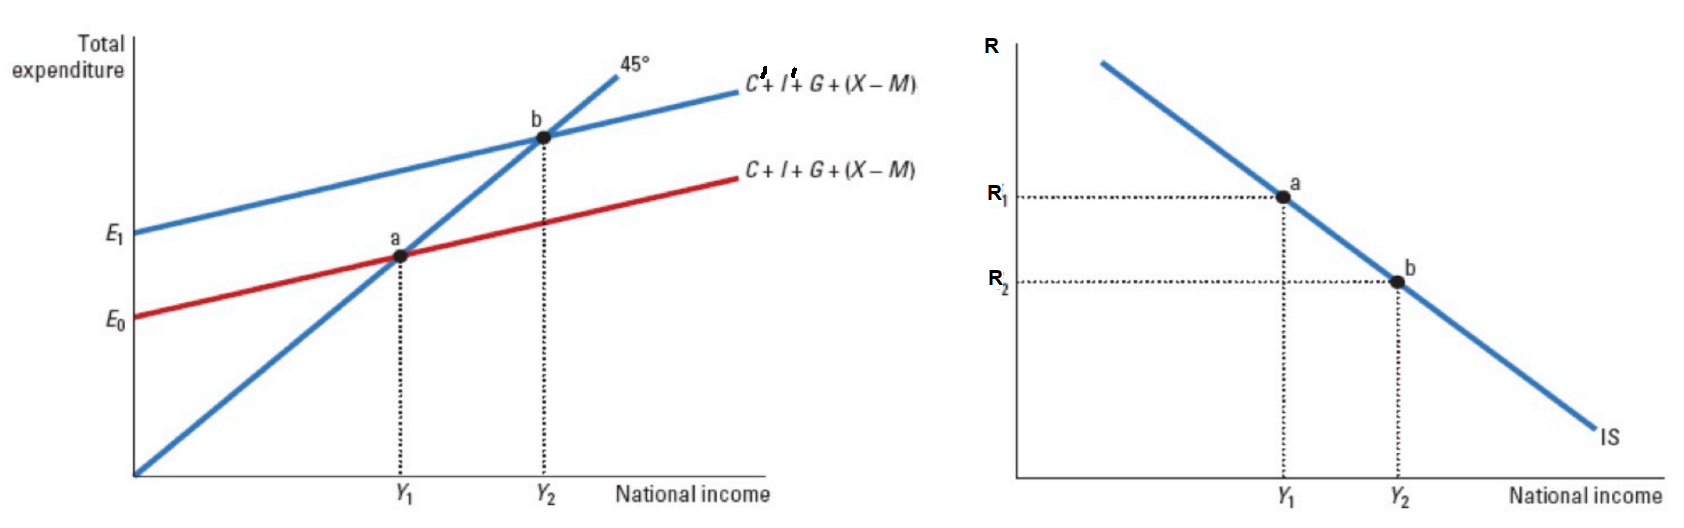
\includegraphics[scale=.25]{deriving_IS_curve}
\end{figure}
\end{frame}

\begin{frame}
\frametitle{\: \: \: Parametric Shifts in the IS-curve}
\toplinelarge
\begin{figure}
\centering
\caption{IS curve: $Y=\left[\frac{1}{1-b_c}\right]* \left[a_c+ a_i-b_i (R) + \overline{G}+\overline{X}-\overline{M}\right]$}
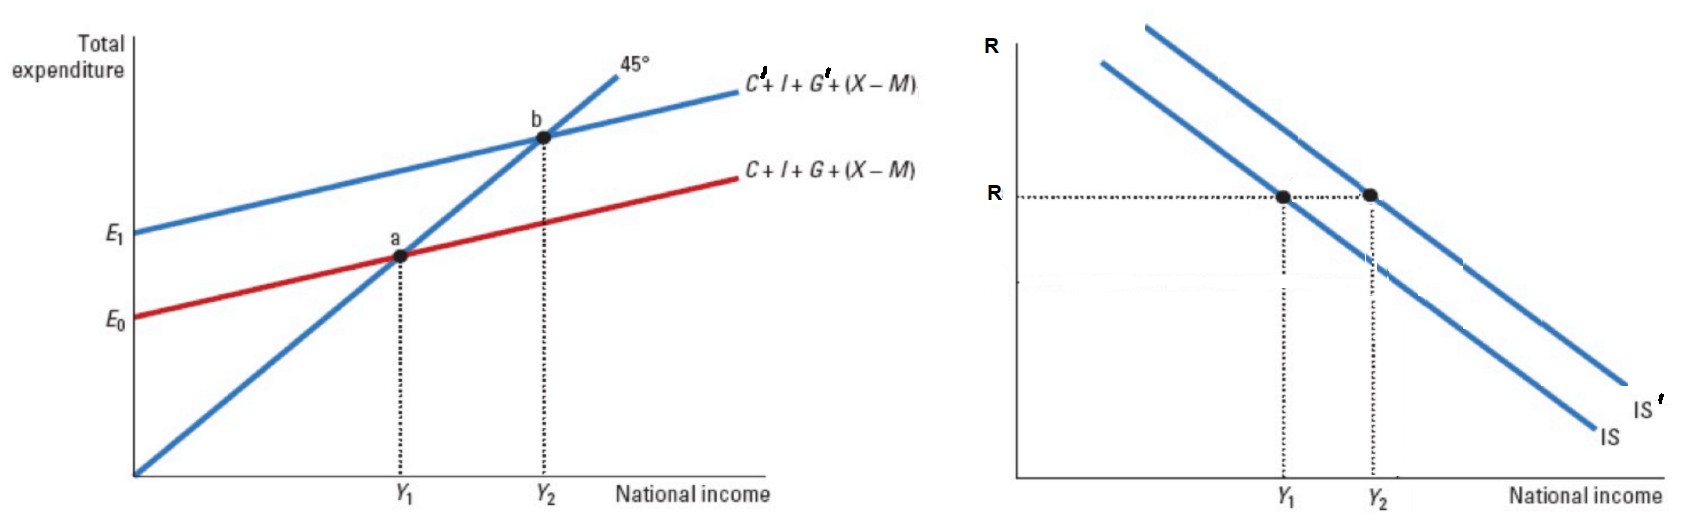
\includegraphics[scale=.25]{parametric_IS_curve}
\end{figure}
\end{frame}


\begin{frame}
\frametitle{\: \: \: Change of scale}\label{scale}
\toplinemedium
\begin{itemize}
\item We are interested in $\widetilde{Y}_t=\frac{Y_t-\overline{Y}}{\overline{Y}}$, so we are going to rewrite the equilibrium as follows:
\begin{eqnarray*} 
\widetilde{Y}_t=\left[\frac{1}{1-b_c}\right]* \left[\overline{a}-\overline{b}_i (R_t-\overline{r}) \right]-1
\end{eqnarray*}
\begin{itemize}
\item $\overline{a}=\frac{a_c}{\overline{Y}}+\frac{a_i}{\overline{Y}}-\frac{b_i}{\overline{Y}}\overline{r}+\frac{\overline{G}}{\overline{Y}}+\frac{\overline{X}}{\overline{Y}}-\frac{\overline{M}}{\overline{Y}}$
\vspace{.16in}
\item $\overline{b}_i=\frac{b_i}{\overline{Y}}$
\end{itemize}
\vspace{.16in}
\item If all exogenous variables are at their long-run equilibrium: 
\begin{eqnarray*}
\begin{array}{lll}
\left[\frac{1}{1-b_c}\right]*\overline{a}=1 &\Rightarrow &\widetilde{Y}_t=\left[\frac{1}{1-b_c}\right][-\overline{b}_i*(R_t-\overline{r})]
\end{array}
\end{eqnarray*}
\end{itemize}
\hyperlink{algebra}{\beamerbutton{Algebra}}
\end{frame}

\begin{frame}
\frametitle{\: \: \: IS-curve with new scale}
\toplinelarge
\begin{figure}
\centering
\caption{IS-curve:$\widetilde{Y}_t=\left[\frac{1}{1-b_c}\right]* \left[\overline{a}-\overline{b}_i (R_t-\overline{r}) \right]-1$, $\overline{a}\left[\frac{1}{1-b_c}\right]=1$}
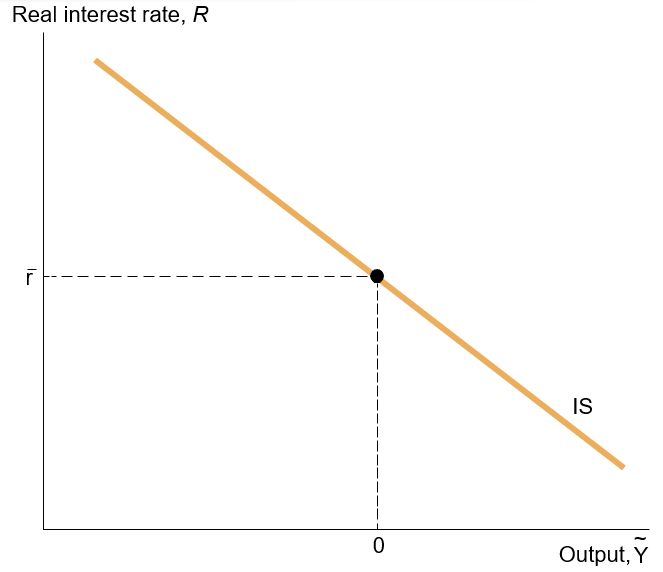
\includegraphics[scale=.5]{IS_curve}
\end{figure}
\end{frame}


\begin{frame}
\frametitle{\: \: \: Changes in the real interest rate}
\toplinelarge
\begin{figure}
\centering
\caption{IS-curve:$\widetilde{Y}_t=\left[\frac{1}{1-b_c}\right]* \left[\overline{a}-\overline{b}_i (R_t-\overline{r}) \right]-1$, $\overline{a}\left[\frac{1}{1-b_c}\right]=1$}
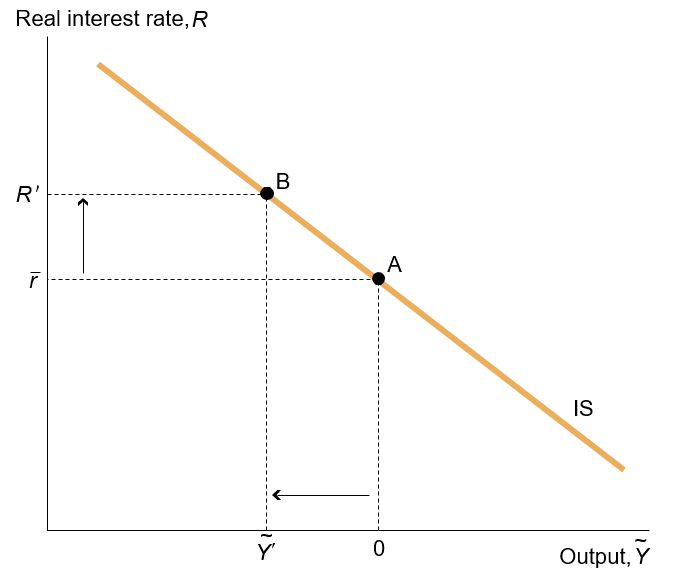
\includegraphics[scale=.5]{IS_curve_interest_rate}
\end{figure}
\end{frame}

\begin{frame}
\frametitle{\: \: \: Temporary Aggregate Demand Shock}
\toplinelarge
\begin{figure}
\centering
\caption{IS-curve:$\widetilde{Y}_t=\left[\frac{1}{1-b_c}\right]* \left[\overline{a}-\overline{b}_i (R_t-\overline{r}) \right]-1$, $\overline{a}\left[\frac{1}{1-b_c}\right]=1$, $\overline{a}'>(1-b_c)$}
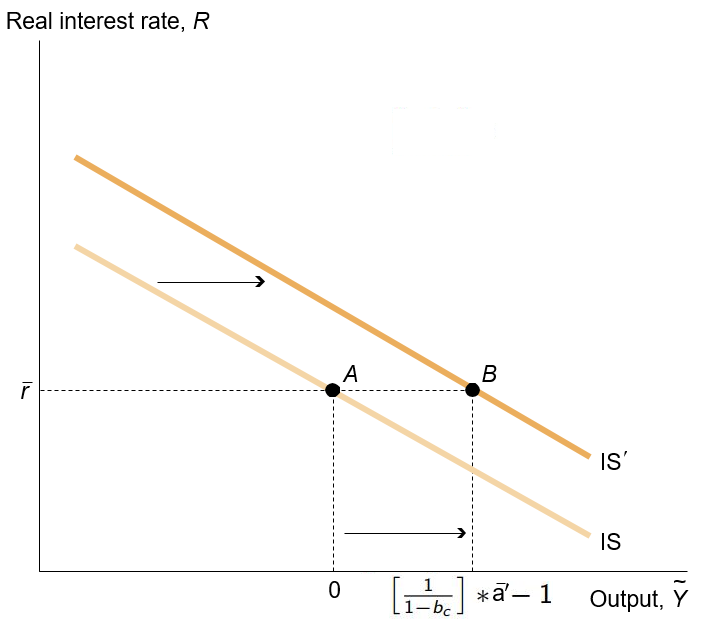
\includegraphics[scale=.39]{aggregate_demand_shock}
\end{figure}
\end{frame}

\begin{frame}
\frametitle{\: \: \: Permanent Aggregate Shock}
\toplinelarge
\begin{itemize}
\item Permanent shocks impact potential output and originate from the production side of the economy, which have two effects:
\begin{enumerate}
\vspace{.11in}
\item Permanent shocks affect demand parameters, which affect both long- and short-run output levels equally.
\vspace{.11in}
\item Permanent production shocks affect the $MPK$
\begin{itemize}
\vspace{.11in}
\item This has no effect in the long-run because $\overline{r}=MPK$
\vspace{.16in}
\item This results in output overshooting in the SR as the economy adjusts to its new potential output.
\end{itemize}
\end{enumerate}
\end{itemize}
\end{frame}

\begin{frame}
\frametitle{\: \: \: E.g. Permanent TFP shock}
\toplinelarge
\begin{figure}
\centering
\caption{IS-curve:$\widetilde{Y}_t=\left[\frac{1}{1-b_c}\right]* \left[\overline{a}-\overline{b}_i (R_t-\overline{r}) \right]-1$, $\overline{a}\left[\frac{1}{1-b_c}\right]=1$, $\overline{r}'>\overline{r}$}
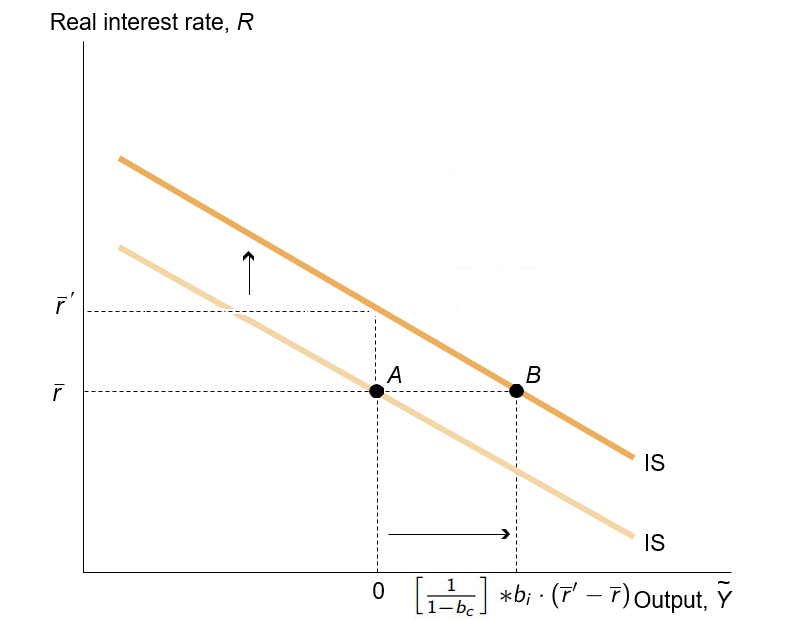
\includegraphics[scale=.39]{permanent_shock}
\end{figure}
\end{frame}


\section{Monetary Policy}

\begin{frame}
\frametitle{\: \: \: Monetary Policy}
\toplinemedium
\begin{itemize}
\vspace{.11in}
\item The BoC currently has three main monetary policy variables at its disposal.
\begin{enumerate}
\vspace{.11in}
\item Overnight rate
\vspace{.11in}
\item Open-market operations
\vspace{.11in}
\item Reserve requirements
\end{enumerate}
\end{itemize}
\end{frame}

\begin{frame}
\frametitle{\: \: \: Overnight rate }
\toplinemedium
\begin{itemize}
\item Overnight rate: The interest rate on very short-term loans between commercial banks.
\vspace{.11in}
\begin{itemize}
\item The BoC can indirectly change the interest rate at which commercial banks lend to each other.
\end{itemize}
\vspace{.11in}
\item When banks lend too much and do not meet the reserve requirement, they are able to borrow short-term from other commercial banks which have excess reserves or from the BoC itself at the overnight rate to meet the requirement.
\begin{itemize}
\vspace{.11in}
\item A high overnight rate encourage banks to lend less.
\end{itemize}
\vspace{.11in}
\item The BoC announces changes in the overnight rate on eight fixed days each year (around every month and a half).
\end{itemize} 
\end{frame}

\begin{frame}
\frametitle{\: \: \: Overnight rate }
\toplinemedium
\centering
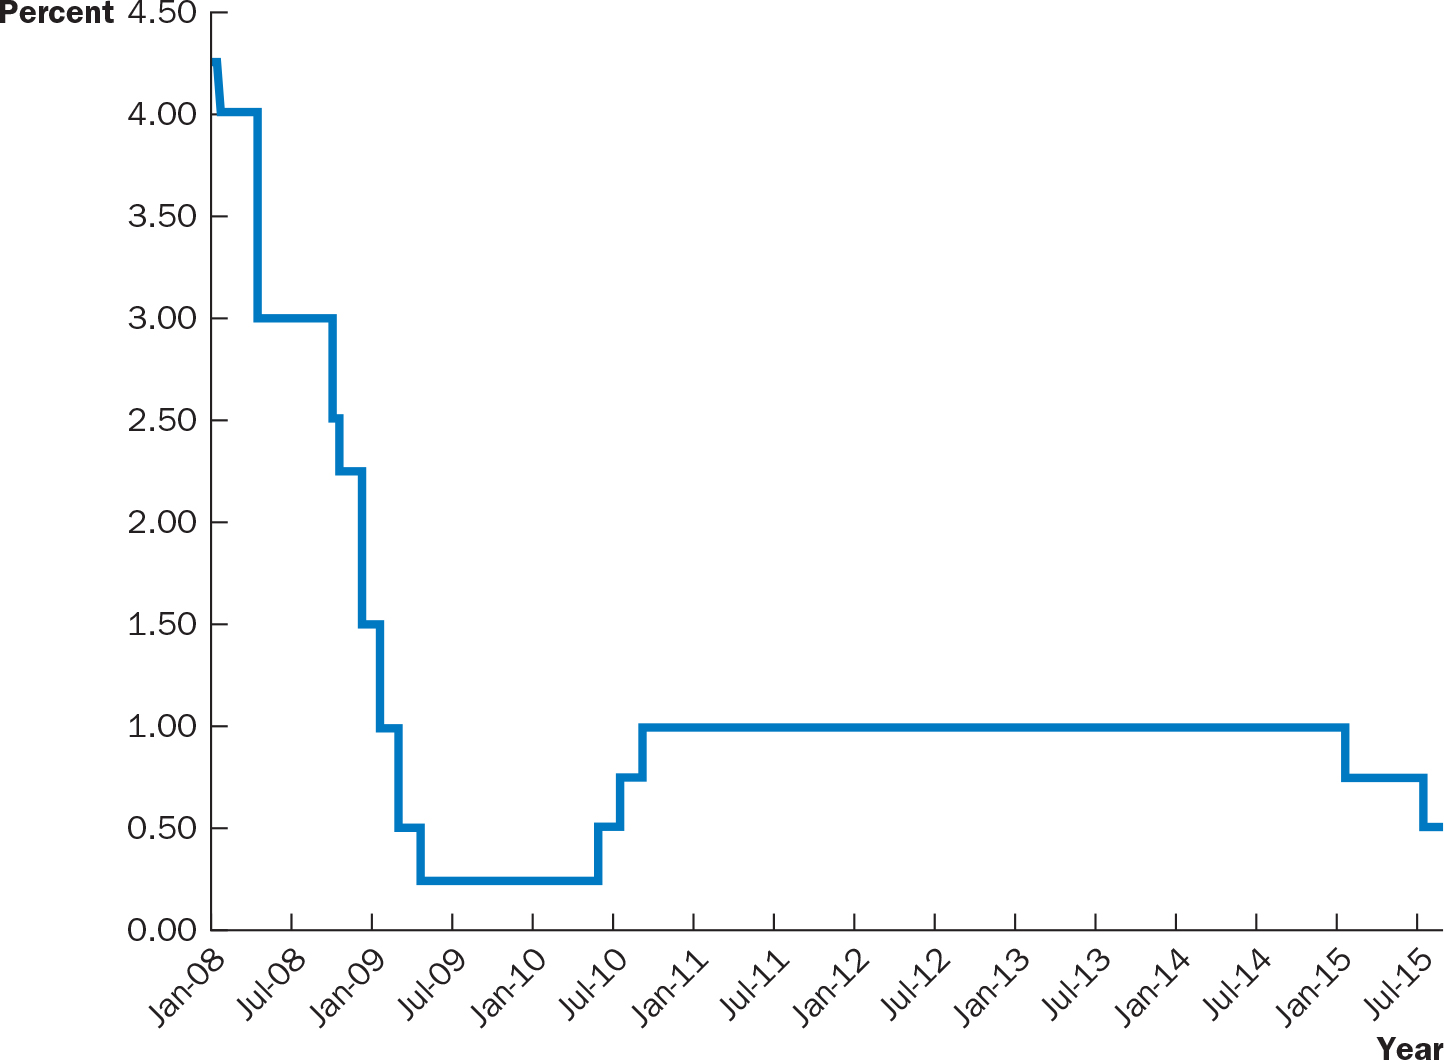
\includegraphics[scale=.8]{overnight_rate.jpg}
\end{frame}


\begin{frame}
\frametitle{\: \: \: From nominal to real interest rate}
\toplinexlarge
\begin{itemize}
\item By modifying the overnight rate, the BoC affects the nominal interest rate in the market.
\begin{itemize}
\vspace{.11in}
\item Commercial banks' additional borrowing costs is pass on to borrowers
\end{itemize}
\vspace{.11in}
\item We can study the effect of changes in the nominal interest rate on the real interest rate using the fisher equation:
\begin{eqnarray*}
R_t=i_t-\pi_t
\end{eqnarray*} 
\begin{itemize}
\vspace{.11in}
\item We are going to assume that in the SR, prices are sticky and only change slowly over time.
\vspace{.11in}
\item In the SR, $\Delta \pi$ do not completely offset $\Delta i$ (this is different in the long-run).
\vspace{.11in}
\item Therefore, in the SR, CB monetary policy has an indirect influence on the real rate return, R.
\end{itemize}
\end{itemize}
\end{frame}

\begin{frame}
\frametitle{\: \: \: The MP curve}
\toplinemedium 
\begin{figure}
\centering
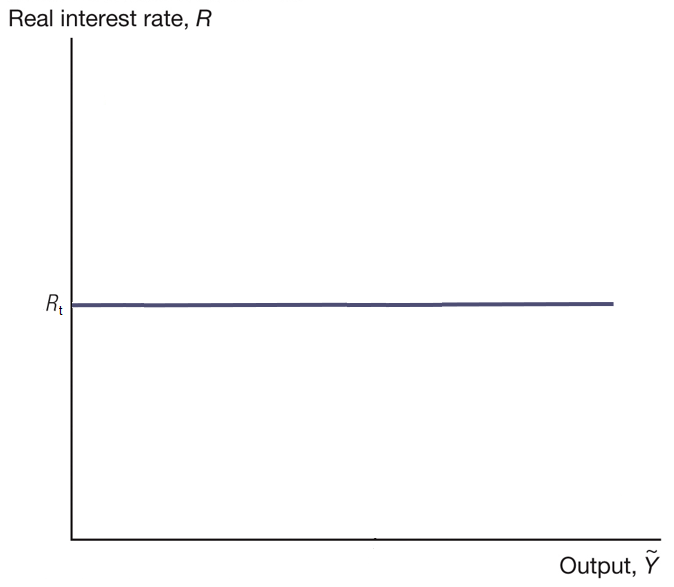
\includegraphics[scale=.4]{MP}
\end{figure}
\end{frame}

\begin{frame}
\frametitle{\: \: \: The IS-MP model}
\toplinemedium 
\begin{itemize}
\item The \textcolor{blue}{MP curve}
\begin{itemize}
\vspace{.11in}
\item Illustrates the central bank's ability to set the real interest rate at a particular value (horizontal line)
\end{itemize}
\vspace{.11in}
\item The \textcolor{blue}{IS curve}
\begin{itemize}
\vspace{.11in}
\item Illustrates the negative reltionship between short-run output and interest rates (through changes in aggregate expenditure)
\end{itemize}
\end{itemize}
\end{frame}


\begin{frame}
\frametitle{\: \: \: The IS-MP model}
\toplinemedium  
\begin{figure}
\centering
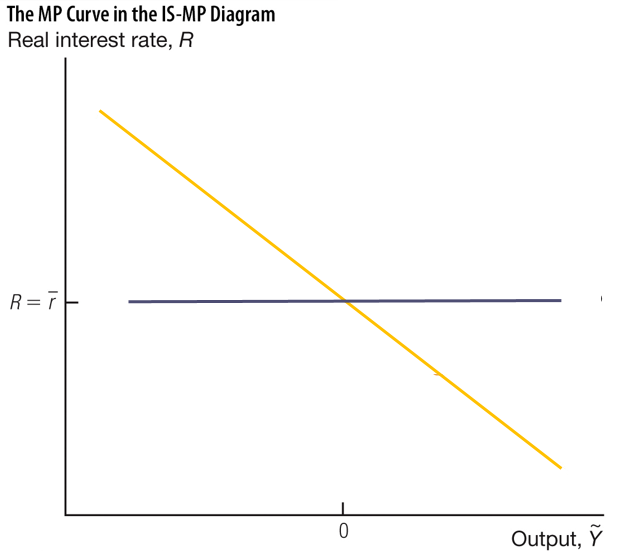
\includegraphics[scale=.5]{IS_MP}
\end{figure}
\end{frame}

\begin{frame}
\frametitle{\: \: \: The IS-MP model}
\toplinemedium  
\begin{figure}
\centering
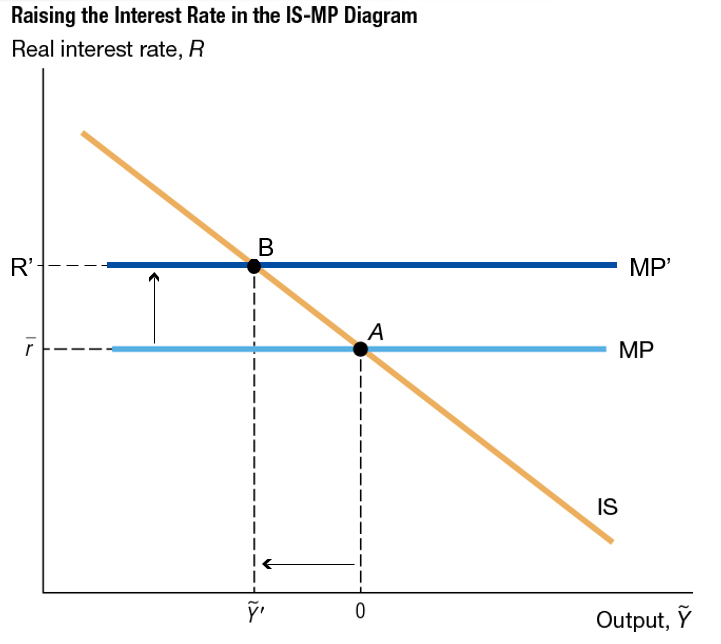
\includegraphics[scale=.46]{IS_MP_interest_rate}
\end{figure}
\end{frame}


\begin{frame}
\frametitle{\: \: \: Temporary Negative Demand Shock}
\toplinexlarge
\begin{figure}
\centering
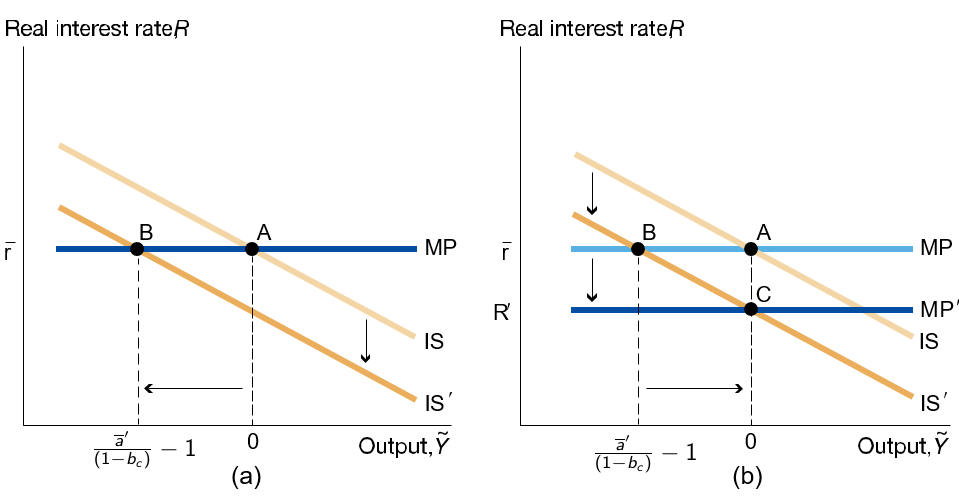
\includegraphics[scale=.46]{temporary_shock}
\end{figure}
\end{frame}

\section{Appendix}

\begin{frame}
\frametitle{\: \: \: Change of Scale: Derivation (part 1)}\label{algebra}
\toplinelarge
\begin{itemize}
\item We begin with the solution to $Y_t$ in the SR equilibrium:
\begin{eqnarray*}
Y_t=\frac{1}{1-b_c} \left(a_c+a_i-b_i \: R_t +\overline{G}+\overline{X}-\overline{M}\right)
\end{eqnarray*}
\item We first divide both sides by the long-run output level $\overline{Y}$ and then subtract one from both sides:
\begin{eqnarray*}
\frac{Y_t}{\overline{Y}}-1=\underbrace{\frac{Y_t-\overline{Y}}{\overline{Y}}}_{\widetilde{Y}_t}=\frac{1}{1-b_c} \left(\frac{a_c}{\overline{Y}}+\frac{a_i}{\overline{Y}}-\frac{b_i}{\overline{Y}} \: R_t +\frac{\overline{G}}{\overline{Y}}+\frac{\overline{X}}{\overline{Y}}-\frac{\overline{M}}{\overline{Y}}\right)-1
\end{eqnarray*}
\item We add and subtract $\frac{b_i}{\overline{Y}} \: \overline{r}$:
\begin{eqnarray*}
\widetilde{Y}_t=\frac{1}{1-b_c} \left(\frac{a_c}{\overline{Y}}+\frac{a_i}{\overline{Y}}-\frac{b_i}{\overline{Y}} \: R_t +\frac{b_i}{\overline{Y}} \: \overline{r}-\frac{b_i}{\overline{Y}} \: \overline{r}+ \frac{\overline{G}}{\overline{Y}}+\frac{\overline{X}}{\overline{Y}}-\frac{\overline{M}}{\overline{Y}}\right)-1
\end{eqnarray*}
\end{itemize}
\end{frame}

\begin{frame}
\frametitle{\: \: \: Change of Scale: Derivation (part 2)}
\toplinelarge
\begin{itemize}
\item We rearrange terms to obtain:
\begin{eqnarray*}
\begin{array}{l}
\widetilde{Y}_t=\frac{1}{1-b_c}\left[\overline{a}-\overline{b}_i \left(R_t-\overline{r}\right)\right]-1  \\
\text{where,}\\
\overline{a}=\frac{a_c}{\overline{Y}}+\frac{a_i}{\overline{Y}}-\frac{b_i}{\overline{Y}} \: \overline{r} + \frac{\overline{G}}{\overline{Y}}+\frac{\overline{X}}{\overline{Y}}-\frac{\overline{M}}{\overline{Y}}\\
\text{and,}\\
\overline{b_i}=\frac{b_i}{\overline{Y}} \\
\text{and,}
\overline{Y}=\frac{1}{1-b_c} \left(a^{LR}_c+a^{LR}_i-b^{LR}_i \: \overline{r} +\overline{G}^{LR}+\overline{X}^{LR}-\overline{M}^{LR}\right)
\end{array}
\end{eqnarray*}
\item From the previous equation, we can see that if all parameters in the SR are equal their long-run levels:
\begin{eqnarray*}
\overline{a}=\frac{a^{LR}_c+a^{LR}_i-b^{LR}_i \: \overline{r}+\overline{G}^{LR}+\overline{X}^{LR}-\overline{M}^{LR}}{\frac{1}{1-b_c} \left(a^{LR}_c+a^{LR}_i-b^{LR}_i \: \overline{r} +\overline{G}^{LR}+\overline{X}^{LR}-\overline{M}^{LR}\right)}
\end{eqnarray*}
\item Solving for this results in: $\overline{a}=1-b_c$
\end{itemize}
\hyperlink{scale}{\beamerbutton{Back}}
\end{frame}


\end{document}

